% The End of All Gears — the pit you climb out of, seen from outside it.
% A cut in the ground with a winding gear over it and nothing else built.
%
% Written by filling in tikz_figure_prompt.md.
\documentclass[tikz,border=4pt]{standalone}
\usetikzlibrary{calc}

% ---- tunables -------------------------------------------------------------
\newcommand{\Unit}{0.055cm}
\newcommand{\Edge}{2.2pt}
\newcommand{\Spokes}{6}        % spokes in the winding gear
\newcommand{\WheelR}{11}       % its radius
\newcommand{\Ground}{22}       % the ground line

\definecolor{slag}{HTML}{5A564C}
\definecolor{slagdark}{HTML}{35322C}
\definecolor{pit}{HTML}{141419}
\definecolor{brass}{HTML}{C08A2E}
\definecolor{ink}{HTML}{101018}

\begin{document}
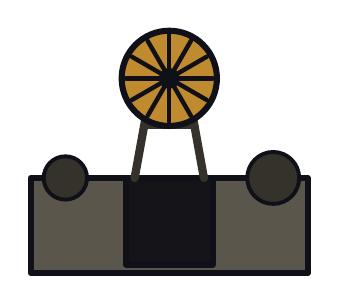
\begin{tikzpicture}[x=\Unit,y=\Unit, line join=round, line cap=round]

  % ---- ground -------------------------------------------------------------
  \fill[slag,draw=ink,line width=\Edge] (0,0) rectangle (64,\Ground);
  % Spoil heaps, because everything that came out of it went somewhere.
  \foreach \x/\r in {8/5, 56/6} {
    \fill[slagdark,draw=ink,line width=1.4pt] (\x,\Ground) circle (\r);
  }

  % ---- the pit ------------------------------------------------------------
  % Drawn over the ground: a hole is an absence, so it is the last thing cut.
  \fill[pit,draw=ink,line width=\Edge] (22,\Ground) rectangle (42,2);

  % ---- the headframe ------------------------------------------------------
  \draw[slagdark,line width=3.0pt] (24,\Ground) -- (28,44);
  \draw[slagdark,line width=3.0pt] (40,\Ground) -- (36,44);
  \draw[slagdark,line width=2.4pt] (26,34) -- (38,34);

  % ---- the winding gear ---------------------------------------------------
  \fill[brass,draw=ink,line width=\Edge] (32,45) circle (\WheelR);
  \foreach \i in {1,...,\Spokes} {
    \pgfmathsetmacro\a{180/\Spokes*\i}
    \draw[ink,line width=1.6pt]
      ($(32,45)+(\a:\WheelR-1)$) -- ($(32,45)+(\a+180:\WheelR-1)$);
  }
  \fill[ink] (32,45) circle (2.4);

  % ---- annotations: none. --------------------------------------------------

\end{tikzpicture}
\end{document}

% ---- self-check ------------------------------------------------------------
% 1. Standalone class, compiles alone with pdflatex.
% 2. Ground height, wheel radius and spoke count are all tunables at the top.
% 3. \foreach draws the spoil heaps and the wheel's spokes.
% 4. Order runs ground -> pit -> headframe -> wheel, so the pit is cut into
%    the ground rather than drawn beside it.
% 5. Rectangles, circles and lines only.
